\begin{figure*}[!ht]
%\begin{subfigure}{0.195\linewidth}
%\centering
%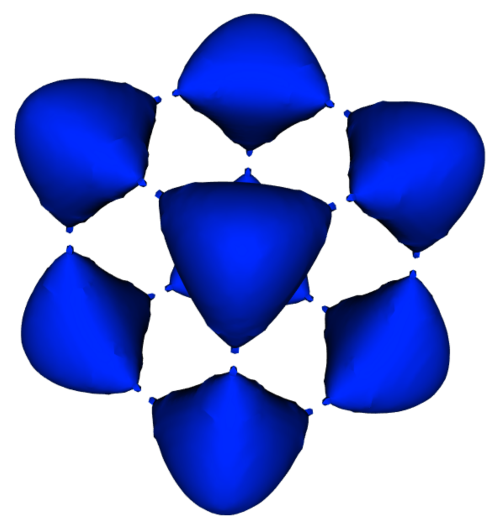
\includegraphics[width=0.85\linewidth]{Images/Tangle/gt.pdf}
%\vspace{-2mm}
%\caption{Ground truth, $isoval=62$}
%\label{fig:tangle_gt}
%\end{subfigure}
\begin{subfigure}{0.19\linewidth}
\centering
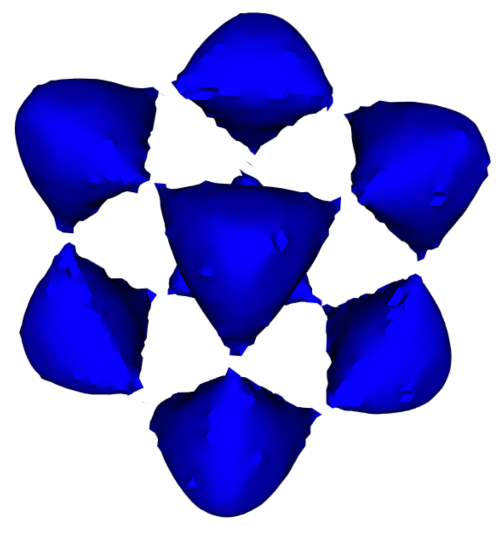
\includegraphics[width=0.9\linewidth]{Images/Tangle/zls.pdf}
\vspace{-2mm}
\caption{$ZLS_{T}$}
\label{fig:tangle_zls}
\end{subfigure}
\begin{subfigure}{0.19\linewidth}
\centering
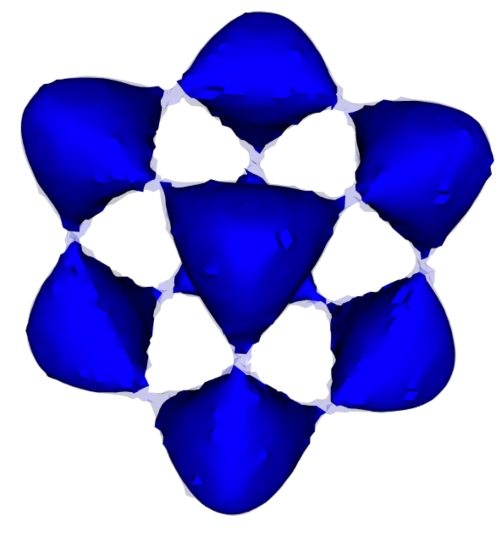
\includegraphics[width=0.9\linewidth]{Images/Tangle/fcls_50.pdf}
\vspace{-2mm}
\caption{+ $FCLS_{T,50\%}$}
\label{fig:tangle_fcls_50}
\end{subfigure}
\begin{subfigure}{0.19\linewidth}
\centering
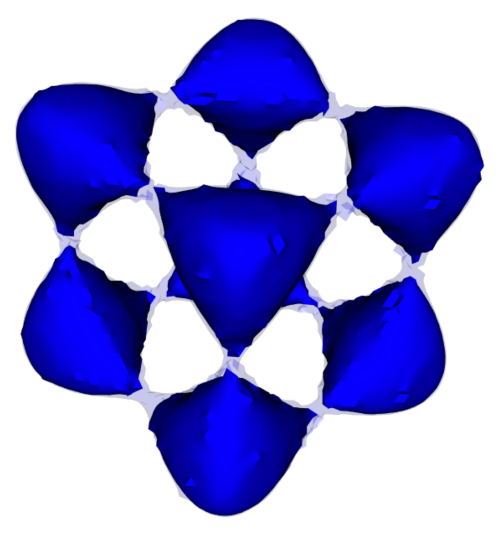
\includegraphics[width=0.9\linewidth]{Images/Tangle/fcls_68.pdf}
\vspace{-2mm}
\caption{+ $FCLS_{T,68\%}$}
\label{fig:tangle_fcls_68}
\end{subfigure}
\begin{subfigure}{0.19\linewidth}
\centering
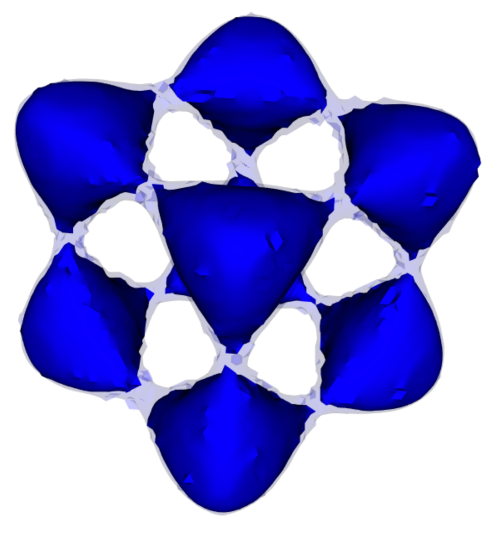
\includegraphics[width=0.9\linewidth]{Images/Tangle/fcls_95.pdf}
\vspace{-2mm}
\caption{+ $FCLS_{T,95\%}$}
\label{fig:tangle_fcls_95}
\end{subfigure}
\begin{subfigure}{0.225\linewidth}
\centering
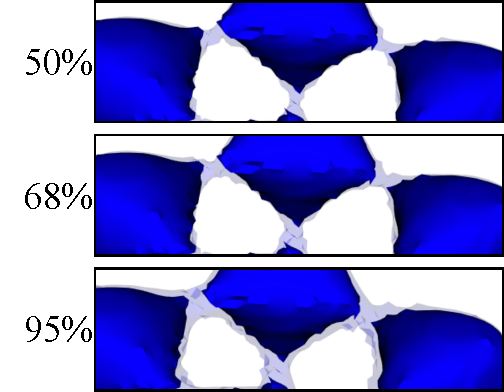
\includegraphics[width=\linewidth, trim={0.2cm 0cm 0cm 0cm}, clip]{Images/Tangle/comparison.pdf}
\vspace{-5mm}
\caption{Comparison of $FCLS_{T,C}$}
\label{fig:tangle_gt}
\end{subfigure}
\vspace{-2mm}
\caption{Visualization of the analytical tangle function with a focus on uncertainty in linking regions between multiple blobs. We used $T=[0,62]$. We use the ``+'' symbol to indicate augmentation to $ZLS_{T}$. As expected for this data set, we found $FCLS_{T,C}$~(visualized as 25\% opacity level-sets) are visible in the linking regions and form wider envelopes as the confidence interval increases from 50\%~(c) to 95\%~(e).} 
%\caption{Visualization of sensitivity of the tangle function near values that form links between the multiple blobs. We use $T=[0,62]$.\fix{start a story}}
\label{fig:tangle}
\end{figure*}
